\documentclass[12pt]{article}

% --------------------
% Basic Packages
% --------------------
\usepackage[a4paper,margin=1in]{geometry}
\usepackage{setspace}
\usepackage{graphicx}
\usepackage{amsmath}
\usepackage{amssymb}

\onehalfspacing

% --------------------
% Title and Author
% --------------------
\title{Intelligent Attack Mitigation Using Deep
Reinforcement Learning in IoT
}
\author{Beerala Dinesh}
\date{}

\begin{document}
	\maketitle
	
	\section{Introduction}
	Due to the fast growth in the Internet of Things (IoT), digital systems have undergone a paradigm shift where devices can easily communicate with each other to provide various services ranging from healthcare applications, smart cities, industry automation, to transport. IoT-based systems incorporate a number of devices that possess limited computing capability; thus, they become extremely susceptible to numerous forms of attacks like Distributed Denial of Service (DDoS), malware dissemination, and intrusion attempts. As IoT systems become more widespread, the use of traditional methods like static rules and signatures becomes inadequate due to the increasing nature of attacks.

Artificial Intelligence (AI) methods have received considerable attention for addressing security issues in IoT-based systems. Although these approaches improve attack identification accuracy, they fail to adapt in real-world settings where attack characteristics keep changing over time. The aforementioned drawback resulted in the utilization of Deep Reinforcement Learning (DRL)\cite{Sewak2023} as an intelligent framework for mitigating attacks. Through constant engagement with their environments, DRL algorithms develop suitable strategies in uncertain situations without any human intervention.

The incorporation of deep reinforcement\cite{Shakya} learning into the security mechanisms of IoT networks creates a paradigm shift in terms of moving from defensive to proactive methods of attack detection and prevention. With the help of reward-based techniques, deep reinforcement learning allows effective responses to anomalies and attacks regardless of the lack of information about potential threat signatures. Therefore, it is well suited to use in large-scale distributed IoT networks. Thus, the subject matter of this paper is the intelligent mitigation of attacks in IoT through DRL.
	\subsection{Evolution of IoT and Security Challenges}
    The advent of IoT technology has enabled the use of billions of devices that work in a constrained environment. Most IoT devices are not equipped with secure protocols, hence becoming vulnerable to any form of attack. Such attacks could be DDoS attacks, theft of sensitive data, and botnets, among others. This becomes complicated due to the growing complexity and magnitude of IoT technology.
    \subsection{Limitations of Traditional and Deep Learning-Based Security Approaches}
    The traditional security measures depend upon rule-based signatures; therefore, they are unable to cope with zero-day and emerging attacks. With the use of machine learning and deep learning algorithms, the detection of attack vectors has become much better due to their learning ability through past data. But one thing that remains unchanged is that these algorithms remain static and need training when a new pattern of attack emerges. They cannot perform sequential decision-making.
    \subsection{Role of Deep Reinforcement Learning in Intelligent Attack Mitigation}
    Deep Reinforcement Learning (DRL) \cite{Asad}is a combination of deep learning and reinforcement learning that helps in making autonomous and adaptable decisions. In relation to IoT security, the DRL algorithms are able to learn and determine appropriate policies based on interaction within the IoT network environment with respect to rewards and penalties for actions taken. This has proved effective for the detection and mitigation of attacks like DDoS, intrusions, and malware propagation within IoT networks.

	\section{Background and Conceptual Foundations}
	To design effective methods of attack mitigation using intelligent technologies in the IoT environment, a detailed knowledge of the underlying technology used in IoT systems is required, as well as a profound knowledge of modern threats of cybersecurity. The IoT architecture consists of many interconnected nodes, including heterogeneous devices, communication channels, and cloud servers. Such an inherent structure of IoT networks is drastically different from traditional computing environments.

Currently, there is no doubt that the implementation of artificial intelligence algorithms in cybersecurity can enhance the ability to detect threats and mitigate attacks in computer networks. Nevertheless, the dynamics of cybersecurity threats in IoT require flexible solutions that are able to continuously adapt in real-time conditions based on the current context without relying on static pre-defined rules or historical data only. In this regard, reinforcement learning algorithms represent one of the most promising approaches that can effectively solve these problems.

In this chapter, the structure of IoT systems will be analyzed. Additionally, the nature of security threats will be discussed. The theoretical background of reinforcement learning and deep reinforcement learning will also be presented.
\subsection{IoT Architecture and Security Threat Landscape}
The IoT architecture typically includes three levels – perception, network, and application levels. While playing different roles in the functionality of the system, these components make it possible for an attack to be performed by the same means, as well. For instance, perception level is comprised of sensors and actuators that collect data about their environment. As the sensors and actuators lack computational capabilities, they are usually equipped with basic security solutions, and, therefore, can be physically tampered.\cite{shaikh}

Network level performs data transmission using different protocols, and it may become a target of eavesdropping and man-in-the-middle attacks. Application level is in charge of processing and analyzing the transmitted data and, as such, becomes vulnerable to data manipulation and other forms of attacks. The growth of the number of devices used by the organization creates more opportunities for cyber attacks on the IoT.

The rise of distributed denial-of-service attack (DDoS), in particular, is linked to the increase in number of deployed IoT devices. The DDoS exploits vulnerabilities of IoT devices and makes them participate in massive attacks.\cite{li}

In addition, the differences in the IoT device types and communication protocols make it difficult to implement standard security measures. The more the IoT network grows, the larger its attack surface becomes, making it easier for attackers to find vulnerabilities in the system. This results in the need for more sophisticated security frameworks to cope with these problems.
\subsection{Fundamentals of Reinforcement Learning and Deep Reinforcement Learning}
In reinforcement learning, an algorithm, also referred to as an agent, makes decisions through interactions with its environment in terms of feedback in form of rewards or penalties. As opposed to supervised learning, which uses labeled data, reinforcement learning involves a trial and error strategy whereby the agent can experiment with diverse action and learn from its experiences to improve future performance. Therefore, the goal of the agent in reinforcement learning is to find an optimal policy that ensures maximum total rewards.\cite{kheddar}

Some of the important elements involved in reinforcement learning include the agent, environment, state, action, and reward. An agent is the decision-maker while the environment represents the system that the agent interacts with to make decisions. State refers to the environment's current status while action refers to decisions that can be taken by the agent. Reward is used by the agent as feedback on the success rate of the action taken.

Deep reinforcement learning entails the use of deep neural networks in reinforcement learning to represent values or policies.\cite{Gueriani_2023}
One of the key advantages of DRL is the fact that it allows for generalization and adaptation to different state changes without requiring any modification in programming. The above advantage makes it possible for the use of DRL in the field of cybersecurity since there are many unexpected attack patterns in cyberspace that cannot be modeled effectively.
\subsection{Role of DRL in IoT Security Systems}
Deep reinforcement learning (DRL) can become an essential tool for ensuring the IoT device's safety through intelligent and adaptive protection algorithms. In particular, DRL allows designing security systems that can flexibly modify their operation depending on the current state of the network and the ongoing attacks. As opposed to rule-based or statistics-based security mechanisms, the former requires pre-designed criteria for classifying events, which are difficult to develop.

DRL-based security\cite{hammad} mechanisms are characterized by their capability to observe a stream of network events in real time and to select the most effective reactions. In general, the reactions taken by DRL agents can be described as network traffic filtering. Specifically, they can block, isolate or modify any network event, depending on how the reward function estimates its contribution to the achievement of particular goals.

The use of DRL can be considered effective in the case of intrusion detection and prevention, DDoS attacks mitigation, and botnet detection. Indeed, such DRL-based solutions can recognize unusual network behavior and filter out any suspicious events. Furthermore, they can effectively respond to the previously unknown types of attacks because their reactions depend on their immediate impact rather than past experience with the similar events.
	

In order to gain a better understanding of the differences between different types of learning techniques in IoT security, the following table provides a comparison of these different types of learning in Table \ref{tab:big_comparison}.
\begin{table}[p]
\centering
\caption{Analysis of Learning Techniques for IoT Attack Detection}
\label{tab:big_comparison}
\renewcommand{\arraystretch}{1.5}
\begin{tabular}{|p{2.2cm}|p{2.2cm}|p{3.5cm}|p{3.5cm}|p{3.5cm}|}
\hline
\textbf{Approach} & \textbf{Learning Type} & \textbf{Working Principle} & \textbf{Advantages} & \textbf{Limitations} \\
\hline

Machine Learning (ML) & Supervised / Unsupervised & Learns patterns from historical data to classify normal and malicious behavior & Simple implementation, efficient for known attacks & Poor adaptability to new attacks, requires retraining \\
\hline

Deep Learning (DL) & Supervised & Uses neural networks to automatically extract features from large datasets & High accuracy, handles complex data patterns & High computational cost, lacks real-time adaptability \\
\hline

Reinforcement Learning (RL) & Reward-based & Learns optimal actions through interaction with environment using reward signals & Adaptive decision making, no labeled data required & Slow convergence, limited scalability \\
\hline

Deep Reinforcement Learning (DRL) & Reward + Deep Neural Networks & Combines RL with deep learning to handle complex environments & High adaptability, real-time decision making & High training complexity, requires large data \\
\hline

Hybrid ML-DL Approaches & Combined & Integrates ML and DL techniques for improved detection accuracy & Balanced performance, improved detection rates & Still lacks adaptability in dynamic environments \\
\hline

DRL-based IDS Systems & Reward-based (Advanced) & Uses DRL agents to monitor and mitigate attacks dynamically & Autonomous learning, handles zero-day attacks & Computational overhead, exploration risk \\
\hline

\end{tabular}
\end{table}
\clearpage
% ---- Figure (Generic Conceptual Diagram)
	\begin{figure}[ht]
        \centering
        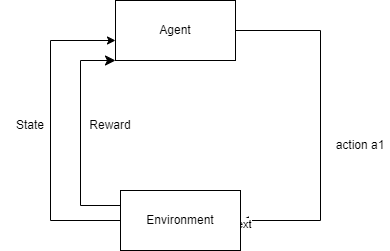
\includegraphics[width=0.95\linewidth]{rl_agent_environment.drawio.png}
        \caption{Deep Reinforcement Learning framework for intelligent attack mitigation in IoT environments. The agent interacts with the IoT network environment by observing states, taking actions, and receiving rewards.}
        \label{fig:drl_iot}
        \end{figure}
	
	

	\section{Core Concepts and Approaches}
	Deep Reinforcement Learning can be considered an essential element in designing intelligent systems for mitigating cyber-attacks in Internet of Things networks because of the inherent uncertainty and unpredictability of these attacks. In contrast to other types of machine learning approaches, Deep RL does not require training based on past data but involves learning optimal behaviors through constant interactions with the surrounding environment. Such properties make Deep RL indispensable for cybersecurity as the nature of attacks constantly changes and, therefore, cannot be predicted using static data.

The concept of DRL enables one to approach the task of attack mitigation from the perspective of sequential decision-making in IoT networks. To achieve effective cyber protection, the system should be viewed as an environment where an agent performs actions and obtains state rewards for its decisions while trying to avoid any potential security threats. DRL is used to enhance an agent's decision-making skills through maximizing the obtained cumulative reward. The following part describes key principles and concepts of using Deep RL for mitigating attacks in IoT networks.
\subsection{DRL-Based Attack Detection and Mitigation Framework}
As mentioned above,\cite{Janakiraman2023} attack detection using Deep Reinforcement Learning presumes the use of an interactive approach, meaning that all security-related decisions must be made taking into account various dynamics observed in real time. Typically, a DRL-based mitigation system consists of three major components: environment, agent, and the learning model itself. In the first case, the environment means the IoT network and its components, whereas the agent means the decision maker that analyses the current network condition and applies appropriate mitigation strategies.

Representation plays a crucial role\cite{LU2024126886} in making the DRL-based learning model efficient. It includes such parameters as packet transmission rates, latency, node behavior, etc. An appropriate state space enables to collect information that will enable to distinguish the normal activity from the attacks. Action space means the list of actions, such as isolation, blocking, rerouting, and so forth.
\begin{figure}[h]
\centering
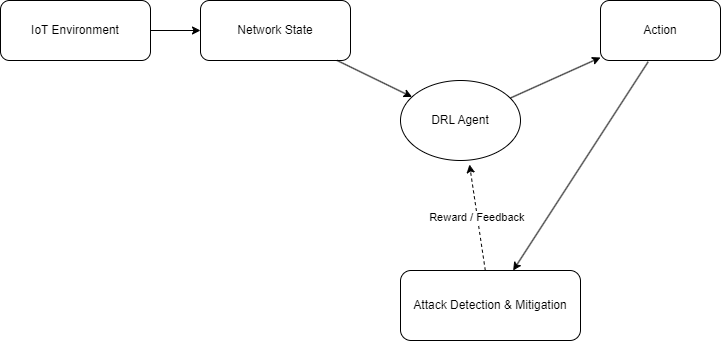
\includegraphics[width=0.75\linewidth]{RNN attack mitigation framework in IoT.drawio.png}
\caption{Deep Reinforcement Learning-based attack mitigation framework in IoT environments, where the agent observes network states and takes actions to detect and mitigate cyber threats.}
\label{fig:drl_framework}
\end{figure}
Reward function is the most significant component of the considered solution since it guides the whole learning process. Reward function can serve several purposes, among which is attack minimization, prevention of false negatives, and optimization of network performance.\cite{alfawa}
\subsection{DRL Algorithms and Learning Strategies}
However, the performance of Deep Reinforcement Learning in IoT cybersecurity\cite{LU2024126886} mainly depends on the selected algorithms and reinforcement learning methods. The Deep Q-network is one of the most commonly used algorithms of DRL with discrete action space. They use the neural network to estimate the function of the Q-value, which shows the expected total reward of making some action within a particular state.

On the other hand, the method of Policy Gradient optimization implies that the policy function is being optimized to allow the agent to learn to choose action distribution probabilistically. It is mostly applicable in cases when there is no discrete action space. Finally, Actor-Critic architecture is applied to combine value-based and policy-based learning.

Finally, there is a variety of techniques that increase the efficiency of DRL applications. Firstly, experience replay technique enables agents to learn from the previous experience. Secondly, target networks are often used in order to avoid fluctuations during the learning process by offering stable references for updating.
Another critical factor is the exploration-exploitation trade-off. The agent needs to find a balance between exploration for discovering optimal policies and exploitation by using the existing actions with the highest rewards. The epsilon-greedy algorithm and the use of entropy regularization methods are typical examples of how to achieve this balance.

In cybersecurity, reinforcement learning models allow the agent to recognize complicated patterns of attacks and react adequately. For instance, in intrusion detection, the algorithm will learn how to classify network activity depending on its behavior patterns. The same applies to DDoS protection when an agent can change filtering rules in order to minimize the influence of attacks and preserve normal traffic.
\subsection{Integration of DRL with IoT, Edge, and Fog Computing}
The incorporation of DRL into IoT networks\cite{R} can be greatly boosted through the application of edge/fog computing paradigms. The traditional approach based on cloud technologies is associated with low efficiency and high latency since it can be difficult to address security threats in real time. To resolve this problem, edge computing enables placing computations closer to the source of the input data.

Edge-based systems allow deploying multiple intelligent agents that process data on-site rather than sending this information to centralized resources. As a result, it will become possible to minimize latency while increasing the efficiency of the IoT networks. Moreover, there will be a possibility of improving privacy since data transmission can be minimized.

The adoption of fog computing will also help to achieve better results through providing additional levels for processing data between the edge layer and the cloud. These layers will facilitate collaboration between multiple agents in order to perform coordinated actions. For example, fog computing nodes will have an opportunity to receive data from different agents and obtain a complete overview of the entire network.
The fusion of DRL with edge and fog computing provides an efficient and scalable system for the security of the Internet of Things. This allows for a process of distributing intelligence whereby the collaboration between several agents can lead to the identification and neutralization of the threats in various segments of the network.
	\subsection{Hybrid DRL-Based Security Models}
    The creation of IoT security\cite{Asad} through the use of DRL-based technology includes developing hybrid approaches that would involve the incorporation of several machine learning approaches with DRL-based technologies to leverage their capabilities.

First of all, it should be mentioned that the use of DRL\cite{kheddar} together with the mentioned machine learning approaches presupposes their implementation in different situations, including the use of machine learning for feature extraction and the use of DRL for decision-making based on the extracted features. In addition, DRL can be integrated into supervised learning approaches since the algorithm trained on labeled data becomes much faster in terms of convergence.

Last but not least, the problem of adversarial attacks in the field of IoT is addressed using hybrid approaches. What is meant by this is that the implementation of adversarial attack can be viewed as a specific case where an attacker tries to manipulate an input data point to ensure its incorrect classification. To protect the IoT system against the attack, it is important to use multiple machine learning algorithms at once to reduce the likelihood of being manipulated.

On the whole, there are many advantages associated with the use of hybrid approaches to DRL.

	\section{Comparative Discussion}
	With the advancement of complexity and sophistication of IoT systems, it becomes necessary to develop smart security measures that can handle dynamic and complex attacks. Some approaches like machine learning, deep learning, and deep reinforcement learning algorithms have been recommended to address this challenge. The differences between these methods lie in their learning mechanisms, adaptability, computational complexity, and performance in handling real-time attacks. Hence, it is important to analyze and assess these approaches in order to determine the most appropriate strategy to secure IoT systems.

Both machine learning and deep learning algorithms have shown tremendous success in identifying previously known attacks through their data-driven nature. However, due to their inability to learn in dynamic situations, these techniques fall short in addressing dynamic attacks. Contrarily, deep reinforcement learning algorithms adopt an interactive and dynamic environment during the learning process. This section of the paper discusses these techniques in detail along with their comparisons.
\subsection{Machine Learning vs Deep Learning in IoT Security}
Traditionally, machine learning\cite{bommana} techniques have been employed for the detection of intrusions and anomalies in IoT networks. Feature extraction along with statistical modeling is involved in classifying network behavior. Decision trees, support vector machines, and clustering algorithms have all been extensively used to detect anomalies in network traffic. Some of the main benefits of using machine learning include lower computational complexity compared to deep learning.

On the other hand, machine learning involves manually engineered features that are often not sufficient for capturing complex relationships within large volumes of high-dimensional data, especially within large-scale IoT networks. Furthermore, machine learning models usually involve training on previous data sets, meaning that they cannot detect new attacks such as zero-day attacks.

On the contrary, deep learning employs the use of neural networks for automatically extracting representations from raw data. Convolutional and recurrent neural networks have become increasingly popular due to their capacity to detect patterns in network traffic.
These techniques, however, come with certain drawbacks that include high computational complexity and the need for massive labeled data. For IoT applications, labeled data may prove expensive and time-consuming, and therefore, it might impact their deployment. Moreover, these methods are static because they use fixed parameters that do not sufficiently adapt to different attack patterns.
\subsection{Deep Reinforcement Learning vs Traditional Approaches}
The primary distinction of deep reinforcement learning from conventional methods is the introduction of a highly adaptive and flexible learning approach. While machine learning and deep learning algorithms learn based on static data sets, DRL\cite{almaraz} models are capable of learning in real-time through interacting with the network and adapting their performance according to changes.

One of the main benefits of deep reinforcement learning is the capability to deal with sequential decision-making problems. When it comes to cybersecurity issues associated with an IoT environment, a mitigation response usually consists of a number of consecutive actions that need to be performed. Thus, mitigating a DDoS attack will require detecting the abnormal traffic, filtering malicious data packages, reallocating resources, and so forth. DRL models are able to learn to perform such sequences in an optimal manner.

Furthermore, DRL is capable of dealing with new and unknown attacks. Since DRL is not dependent on labelled data, it enables an algorithm to try out new strategies and learn new ways to respond to threats even when there is no previous data available regarding such situations.

\begin{table}[h]
\centering
\caption{Comparison of ML, DL, and DRL Techniques for IoT Attack Mitigation}
\label{tab:comparison_methods}
\renewcommand{\arraystretch}{1.5}
\begin{tabular}{|p{2.5cm}|p{3cm}|p{3cm}|p{3cm}|}
\hline
\textbf{Criteria} & \textbf{Machine Learning} & \textbf{Deep Learning} & \textbf{Deep Reinforcement Learning} \\
\hline
Data Requirement & Moderate labeled data & Large labeled datasets & Interaction-based learning \\
\hline
Adaptability & Low & Moderate & High \\
\hline
Real-time Response & Limited & Moderate & High \\
\hline
Handling Unknown Attacks & Weak & Moderate & Strong \\
\hline
Computational Cost & Low & High & Very High \\
\hline
Learning Approach & Static & Static & Dynamic \\
\hline
Decision Making & Predictive & Pattern-based & Sequential and adaptive \\
\hline
Suitability for IoT Security & Basic detection & Advanced detection & Intelligent mitigation \\
\hline
\end{tabular}
\end{table}
As is clear from Table \ref{tab:comparison_methods}, DRL is better than traditional machine learning and deep learning techniques when it comes to adaptability and decision making in real time. Although machine learning and deep learning can be used to detect any known threat in the form of an attack, there is not enough room left for them to adapt themselves to any new threats that come up.
\subsection{Performance Evaluation and Scalability Analysis}
One of the essential criteria for the efficiency analysis of security solutions is the evaluation of performance. Performance measures include detection accuracy, false positive rate, response time, and computational load. The performance of machine learning models includes fast responses and low computational costs, which allows their implementation in lightweight IoT devices. At the same time, machine learning algorithms' low adaptiveness hinders the efficiency in a dynamic environment.

In contrast, deep learning models demonstrate high accuracy, but at a cost of considerable computational load. This model type requires heavy computation and powerful hardware to operate and, thus, does not provide a scalable solution.

Deep reinforcement learning models demonstrate better performance because of constant policy improvement due to interaction with the environment. Moreover, DRL models are scalable when combined with edge or fog computing.

The need for scalability emerges with increasing numbers of IoT devices and generated data. In particular, scalability is critical in implementing security mechanisms for smart cities and other applications where there are many thousands of IoT devices generating large amounts of data.
	

	\section{Practical Insights and Use Cases}
	The use of Deep Reinforcement Learning for the purpose of securing IoT is certainly a huge step forward in the realm of developing smart, autonomous, and adaptive security measures. While many approaches and models are purely theoretical in nature, IoT security faces many challenges, ranging from constrained computational power, unstable network conditions, to varying characteristics of devices. In order to overcome these limitations, it is necessary to come up with practical applications of DRL in IoT security.

There have already been successful attempts at using DRL in the implementation of an attack mitigation system. Such systems have been successfully used in various applications in areas such as healthcare, smart cities, IoT industry, and edge computing. This paper will further investigate some of these practical applications of DRL in IoT security.
\subsection{DRL in Healthcare IoT (IoMT) Systems}
Healthcare IoT systems, commonly referred to as Internet of Medical Things (IoMT), include connected devices, sensors, and monitoring systems used in collecting and exchanging sensitive data related to patients' health conditions. Being highly dependent on wireless communications, IoMT systems are also considered to be extremely vulnerable to cyber threats and attacks, which may lead to various complications, such as interruption of the provided services and violation of the patients' well-being.

Several approaches for addressing security issues in healthcare systems based on deep reinforcement learning (DRL) were offered recently. DRL agents used in IoMT settings perform monitoring of the network traffic and analyze any possible signs of malicious activity. If a threat is detected, an appropriate action can be taken by the agent, including device isolation, traffic filtering, or changing network resources allocation.

A major benefit associated with applying DRL-based security solutions in healthcare is the possibility to provide real-time protection and respond quickly to emerging threats. The DRL-based intrusion detection system can constantly train itself based on its interactions with the network, thereby improving its performance continuously.
\subsection{DRL in Smart Cities and Large-Scale IoT Systems}
	Smart cities constitute some of the most challenging IoT applications, where numerous interrelated systems, including traffic management systems, energy grid systems, public safety systems, environmental monitoring systems, etc., produce huge volumes of data. Moreover, smart cities require advanced protection systems in order to prevent cyberattacks that could compromise critical infrastructures.

One of the areas of intensive research into using deep reinforcement learning algorithms is cybersecurity for smart city IoT systems because of their capability to operate in large and dynamically changing environments. In this regard, a DRL-based algorithm can monitor the IoT network traffic, detect abnormal patterns that may indicate an ongoing attack, and manage the response to ensure the operation of smart city infrastructure.

Another important factor that makes distributed computing architectures effective for smart cities is DRL. The deployment of a number of DRL agents on various levels of the computing architecture would enable the implementation of a coordinated security strategy. It will ensure a prompt reaction to any threats while increasing the scalability of the network.

Additionally, the use of DRL-based algorithms allows addressing another critical issue – resource optimization amid ensuring network security.
\subsection{DRL in Industrial IoT (IIoT) Systems}\cite{Devi}
DRL algorithms for securing IIoT systems are applicable in different areas such as production, energy generation, and critical infrastructure industries. These industries require IoT-based technology due to their scale and demand. In addition, any attacks on systems within the selected industries can bring financial damages, lead to malfunctioning of industrial devices, and create safety concerns.

There are several methods based on DRL algorithms used for protection of IIoT systems from possible attacks. The algorithm examines the behavior of the selected system and its interactions with the outer environment in order to recognize any cyberattacks. The detection of an attack allows the algorithm to react by taking appropriate action such as isolation of affected elements of the system, adjustment of its parameters, or emergency procedure activation.

One of the difficulties in using cybersecurity in the industry lies in balancing cybersecurity measures and functionality of the system. DRL algorithms help solve this issue because they have the ability to optimize several aspects at once. It means that DRL models allow maximizing cyberattack detection while minimizing false alarms.
\subsection{DRL in Edge and Fog Computing Environments}\cite{far2025artificialintelligencesecuredinformation}
With the advent of edge computing and fog computing architectures, it is now possible to distribute computations and process information at different computing nodes to achieve improved real-time security in IoT systems. The adoption of DRL models within such architecture could help improve the performance of DRL models for detecting and mitigating cybersecurity threats.

DRL agents in edge-computing architectures are placed in IoT devices or even gateways within the same premises where network communications are performed. Therefore, the use of such DRL-based models would lead to real-time threat detection and mitigation without necessarily transmitting all data to the central server. In case there is a DDoS attack detected, the DRL-based solution will mitigate the attack locally without spreading it further.

In fog computing, the architecture involves additional layers between IoT devices and the server in order to coordinate the efforts of several DRL agents. For example, the data transmitted from edge devices will first be collected at fog nodes where the pattern recognition task can be completed. Consequently, the data sent to the server would only include the threat information.

Through a combination of DRL models and edge/fog architectures, it is possible to develop more robust cybersecurity solutions for IoT systems.

	\section{Challenges and Open Issues}\cite{OrtegaFernandez2023}
	However, there are certain challenges and obstacles regarding the utilization of reinforcement learning for mitigating cyber attacks, which should be taken into consideration. Given that the environment in which IoT devices operate is characterized by its dynamics and constraints, it can be quite difficult to design such techniques that will be able to generate the needed results. While there are some positive points regarding the use of DRL, at the same time, there are also some drawbacks.

In addition, the employment of this approach within the framework of the IoT network may face a number of difficulties related to the specific features of such systems, including high latency and energy consumption, and heterogeneity. These are just a few of the issues that will need to be addressed prior to implementing reinforcement learning in order to enhance IoT security.
\subsection{Computational Complexity and Resource Constraints}
One of the main drawbacks linked to DRL-based IoT security solutions is their high computational complexity. DRL methods generally require high computational capabilities in order to work properly. It is a significant problem in IoT systems as most of the devices operating in this type of network lack the required hardware capacity to perform complicated operations.

Training of DRL algorithms is connected to an interactive approach involving repeated interaction with the environment. This process is time-consuming and difficult in terms of the required hardware resources that can be unavailable in some cases due to limited device capacity. It creates an obstacle on the way to implementing DRL-based IoT systems since the technology cannot reach its full potential under such conditions.

Another important factor to consider in the context of IoT is energy consumption. Devices in an IoT network are mostly battery-operated and, therefore, should not be used too intensively. Continuous work of DRL algorithms would increase their energy consumption making IoT devices useless very soon. This means that there is a need to optimize existing approaches and develop new algorithms to implement DRL models.
\subsection{Data Scarcity and Training Challenges}
Another important difficulty with using deep reinforcement learning algorithms in the IoT security realm is related to a lack of good training data. As compared with the supervised learning paradigm, where there are many labeled data sources, training data used for reinforcement learning is collected through interactions with the environment over time.

A shortage of relevant data makes it harder for deep reinforcement learning algorithms to achieve satisfactory generalization to different settings and various kinds of attacks. In addition, the process of creating simulated environments and carrying out experiments in such an environment does not reflect real-life conditions accurately and may lead to inferior performances in practice.

Moreover, IoT data often contains noise, making the training process less stable and prone to divergence. Another problem associated with DRL is connected to the need to balance exploration and exploitation. Exploration means trying out new tactics, while exploiting involves applying what has already been learned by the agent.
\subsection{Scalability and Heterogeneity of IoT Networks}
Heterogeneity of IoT networks is another important issue in the development of a DRL framework for purposes of security. This heterogeneity in terms of capability of the nodes, the communication protocol in use, and the operating environment forms one of the greatest impediments towards building the best possible model that works in all conditions.

Scalability of any DRL-based model developed for security is another key consideration while trying to build such models in IoT networks. Since in most cases, the IoT networks comprise of hundreds or even thousands of nodes, it would be difficult to implement DRL in a centralized manner. A distributed approach using fog and edge computing can prove to be a better option in terms of scalability, though coordination among the agents can be a problem.

Lastly, dynamicity remains another challenge towards building a DRL-based security model for the Internet of Things.
\subsection{Security and Robustness of DRL Models}
Though DRL is being used to improve the security of systems, several attacks can be launched against it. Attacks such as adversarial and poisoning attacks can exploit any vulnerability in the models. An adversarial attack means manipulating the input to make the model wrong. This poses a huge challenge because DRL can become a target of attacks when working to protect the Internet of Things from attacks.

Reliability guarantees are also missing in DRLs because the policy adopted is often learnt by the system. This poses a huge risk in using such a methodology in different environments, hence there should be a need to provide guarantees of reliability for such models.

Transparency should also not be ignored as we shall require explainable AI to understand how the models operate.

	\section{Future Directions}
	However, with cyber attacks becoming complex and evolving at a very fast pace, it is essential to keep developing advanced intelligent security solutions as well. It seems that there are still many research directions worth exploring, given that Deep Reinforcement Learning has already shown its potential as an attack defense mechanism that can be used autonomously.

With the increasing growth of IoT ecosystems in industries ranging from healthcare to smart cities and beyond, the demand for intelligent, decentralized, and resilient security solutions continues to grow. In this section, some future research directions in this area will be discussed.
\subsection{Integration of DRL with Emerging Technologies}
One of the most promising areas of future research is related to the combination of DRL with other technologies that emerged recently. Blockchain technology can improve the security and transparency of the IoT system through decentralization and the ability to maintain an immutable database. Blockchain can be used along with DRL to store learning experience safely, exchange information about threats, and make distributed learning secure.

Federated learning also holds great promise because this technology enables several IoT devices to train the DRL algorithm in a collaborative manner without disclosing sensitive data. Combining DRL and federated learning would enable researchers to design distributed intelligence systems capable of operating in various conditions and protecting the data privacy of IoT devices.

Edge intelligence is yet another area of great interest because it allows DRL models to function autonomously in an IoT environment. Future research should look into how to optimize DRL algorithms for functioning in the edge environment where low latency is required.	
\subsection{Development of Lightweight and Efficient DRL Models}
Some of the challenges that have emerged with the application of DRL in IoT systems are the extensive computations and energy requirements of deep learning models. Future research efforts must concentrate on developing lightweight DRL models that would facilitate computations irrespective of the resource-constraints imposed by the computing devices. Methods like model compression, model pruning, and quantization could be explored for building simple yet effective DRL models.

Learning techniques that reduce computational complexity without hampering the efficiency of the computations could emerge as another potential topic for research. Such a technique could ensure that IoT-based systems learn faster while minimizing the drain on battery power of the computing devices. Other methods like transfer learning and meta-learning could help in reducing data acquisition times as well.

All these research topics could be helpful for achieving higher acceptability of DRL-based solutions in IoT.
\subsection{Enhancing Robustness and Security of DRL Models}
Given the growing popularity of DRL-based systems, the issue of making them resilient towards attacks and system failures arises. Thus, future studies should be devoted to the problem of creating robust DRL models.

One of the possible ways to make DRL-based solutions resilient against attacks may be related to adversarial training. Adversarial training refers to the procedure of exposing DRL algorithms to malicious cases to make them stronger. Additionally, ensemble learning may be regarded as another promising approach.

In addition to making DRL models robust, explainability may also be considered as one of the future trends in developing DRL-based approaches to security problems. Given the increasing importance of explainable AI, researchers will be able to create more reliable DRL algorithms.
	\section{Conclusion}
	As for the growing popularity of DRL-based technologies, the question of making such technologies resistant to attacks and failures is becoming urgent. Therefore, it is worth considering this aspect in the course of further research.

One of the potential approaches to ensuring that DRL-based solutions will resist attacks might be associated with the use of adversarial training techniques. As can be seen from the term itself, adversarial training means exposing DRL to adversarial cases in order to make it more resilient. Another approach, such as ensemble learning, can also be mentioned.

Apart from the idea of developing more resilient DRL-based technologies, explainability can also become one of the main directions of further research in this field. With regard to the growing popularity of explainable AI, DRL can also benefit from this.
However, despite the wide range of benefits, there are also several disadvantages associated with DRL, which may negatively impact the performance of IoT security frameworks relying on it. Specifically, some of the main challenges include computational complexity, the lack of training data, scalability issues, and vulnerability to adversarial attacks. Therefore, addressing all of them will allow enhancing the performance of DRL-based solutions in IoT.

There are also multiple possible areas for future developments in this direction. First, integrating DRL algorithms into other emerging technologies such as blockchain, federated learning, and edge intelligence appears to be especially fruitful. Furthermore, developing efficient and robust models capable of operating in constrained environments becomes more relevant. Finally, autonomous and self-healing security frameworks may represent one of the most interesting breakthroughs in this field in the coming years thanks to deep reinforcement learning.

Overall, DRL can become the core element of the future IoT security architectures because of its unique capabilities. The ability to learn new patterns, respond to threats and situations dynamically, and create effective responses allows DRL to become an extremely useful technology.
	

	\bibliographystyle{plain}
	\bibliography{references}
	
\end{document}
